\subsection{Cabibbo Angle}
 It was found that the 
 theory of weak interactions explained well many features of quark and
 of leptonic decays. However, it appeared that the interaction
 strength in quark decays was less than one would expected, especially
 the strange quark seemed to be very reluctant to decay.

 To solve this problem, Cabibbo proposed that the down and the strange
 quark ``share'' the interaction strength/transition amplitude to the
 up quark \cite{cabibbo}. The idea is that there is a particle
 \emph{like} the down quark (let's call it $d^{\prime}$) that couples
 with the expected strength to the up quark, but is in fact a
 superposition of the physical $d$ and $s$ quark.
 \begin{equation}
     d^{\prime} = \alpha d + \beta s
 \end{equation}
 Normalising the $d^{\prime}$ wave function leads to the condition that $\alpha^2 + \beta^2=1$. This is fulfilled by:
 \begin{equation}
 d^{\prime} = \cos\theta_C \, d + \sin\theta_C s
\end{equation}
where $\theta_C$ is the Cabibbo angle (experimentally $\theta_C = 0.22$).
In this scheme, a $d^{\prime}, u, W$ vertex has the same coupling strength ($g_W$) as an $e, \nu_e, W$ vertex. 
But in reality, we do not observe $d^{\prime}$, but the physical $d, s$ quarks ("physics" meaning that they have well defined masses. 
The amplitude for a $d^{\prime}$ become a $d$ quark is $\braket{d^{\prime}}{d} = \cos\theta_C$. Similarly $\braket{d^{\prime}}{s} = \sin\theta_C$.
 So the transition amplitude for $d \to u$ transitions is $\propto
 \cos\theta_C$ and for $s\to u$ transitions it is $\propto \sin\theta_C$
 (Remember that rates are $\propto |\mathrm{amplitude}|^2$).
 
\begin{figure}
\caption{The Cabibbo Angle.\label{fig:cabRot}}
\begin{tabular}{cc}
\parbox{0.45\textwidth}{
The down-type quarks that couple via the $W^{\pm}$ to the up-type quarks are rotated relative to their mass
eigenstates.}
&
\parbox{0.45\textwidth}{
The $W^{\pm}$ can induce a transition $u\to d'$. The transition amplitudes to the mass eigenstates $d, s$  are $\propto$ the
projections of the mass eigenstates onto the $d'$.
}
\\
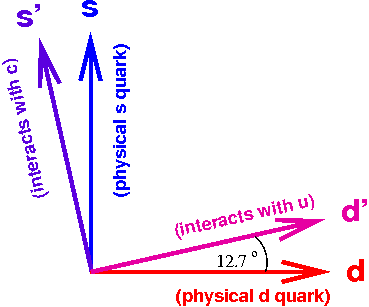
\includegraphics[width=0.45\textwidth]{fig/C_P_CP/cabibboAngle.png}
&
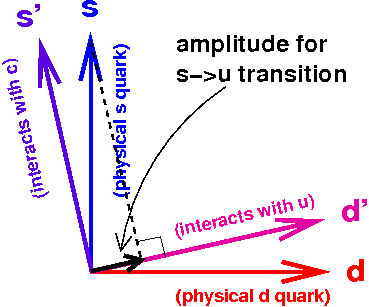
\includegraphics[width=0.45\textwidth]{fig/C_P_CP/cabbibo_with_su.png}
\end{tabular}
\end{figure}
 For symmetry reasons, let us also define an $s'$ such that $d', s'$ are simply rotates states of $d, s$ (this is somewhat anticipating the addition of the charm quark below - an $s'$ doesn't really make sense unless it is the partner of 2nd up-type quark):
 \begin{equation}
   \label{eq:dprime_sprime_trans}
\vII{d^{\prime}}{s^{\prime}} = \mII{\cos\theta_C}{\sin\theta_C}
                                  {-\sin\theta_C}{\cos\theta_C}
\vII{d}{s}
\end{equation}
as illustrated in \figref{fig:cabRot}.

The introduction of quark mixing explained the observed
 $s\leftrightarrow d$ and $u \leftrightarrow d$ couplings, and related them to $W^{\pm}$ couplings in the lepton sector.
 
 So the vertex factors are now:\\
 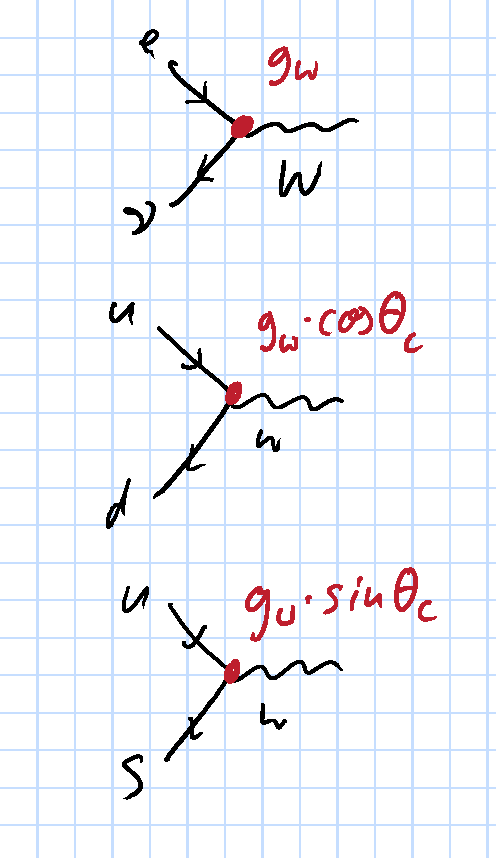
\includegraphics[width=0.5\textwidth]{fig/weak/gWCabibbo}
 
 So instead of three coupling constants, we have one coupling constant
 $g_W$ and one angle, $\theta_c \sim 13.02^{\circ}$ - that is one
 fewer parameter. Describing nature with fewer parameters is usually a
 sign of progress in our understanding of it.
 
 Note that, while $u \leftrightarrow s$ and $u \leftrightarrow d$
 transitions are allowed, no vertices for $s \leftrightarrow d$
 transitions are allowed (even though there is a neutral $Z$ boson
 that could take care of the charge conservation). This is explored a
 bit more deeply in the Appendix~\ref{sec:tree_fcnc}.

\section{New Physics in 1963: Discovery of charm}
 (1963, quarks known at the time: $u, d, s$)\\ In the previous
chapters you learnt about the evidence for the existence of three
quarks, which beautifully described the otherwise messy picture of the
mesons and baryons observed. The key aspects of the theory of weak
interactions (that you also learnt about last year), were also
developed at a time when only three quarks were known: $u, d, s$. The
4th quark, charm, was predicted from observations made in decays of
Kaons. Note that this is quite remarkable. Kaons have a mass of less
than \un{0.5}{GeV}, while the charm quark has a mass of \un{1.3}{GeV}
-- so how can you see a charm quark in a Kaon decay? With this
section, we introduce an important general principle of an approach
that is called "flavour physics": The discovery of "new physics" at
mass scales beyond those of the particles that can be directly
produced and observed, using precision measurements.


\subsection{Flavour changing neutral currents at loop level}
\begin{figure}
\centering
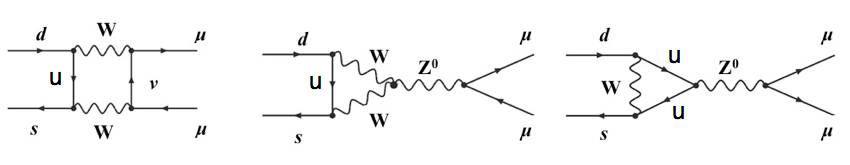
\includegraphics[width=0.9\textwidth]{fig/0_K2mumu1}
\caption{Diagrams contributing to the "Flavour Changing Neutral Current" (FCNC) transition \prt{K^0 \to \mu^+ \mu^-} (w/o GIM cancellation) leading to predicted rates far higher than observed. It is an FCNC because it is a $d-s$ annihilation, so a $d$ couples (indirectly) to an $s$ which has the same charge.
\label{fig:K2mumu1}}
\end{figure}
 The theory as it stands now has one substantial problem suffered from
 one problem, and that was the prediction of ``Flavour Changing
 Neutral Currents'', or FCNC, transitions where the quark flavour
 changes, but not the charge, like $d\to s$.  With the advent of the
 Standard Model of particle physics we know these were already
 impossible at tree level, but loop diagrams such as those in
 \figref{fig:K2mumu1} for the process \prt{K^0 \to \mu^+\mu^-} are
 still possible. This had never been seen and the predicted rate for
 this process was far greater than the observed limits at the time.
 

\subsubsection{GIM}
\begin{figure}
\centering
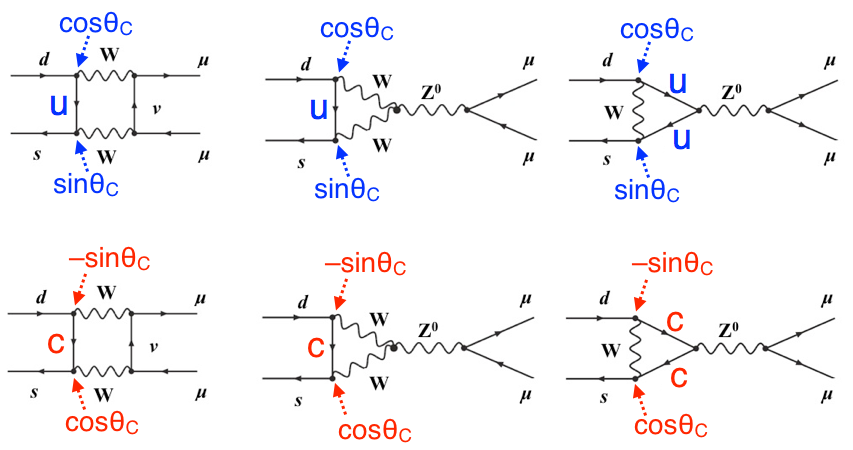
\includegraphics[width=0.9\textwidth]{fig/0_K2mumuGIM}
\caption{GIM mechanism illustrated for the "Flavour Changing Neutral Current" transition \prt{K^0 \to \mu^+\mu^-}. The diagrams resulting from the newly predicted $c$ quark exactly cancel the diagrams with the $u$ quark in the loop. Well - nearly exactly. The mass difference between the $c$ and the $u$ quark leads to slightly different values for the $u$ and the $c$ quark loop diagrams, so while \prt{K^0 \to \mu^+ \mu^-} is highly suppressed, it is not completely forbidden. This effect can even be used to estimate the $c$ quark mass. This mechanism works for any FCNC involving the first two generations (we'll deal with the third generation, soon).
\label{fig:K2mumuGIM}}
\end{figure}

 To explain the absence of flavour changing neutral currents
 S. L. Glashow, J. Iliopoulos and L. Maiani (``GIM'') proposed the
 existence of a fourth, undiscovered quark, the charm quark
 \cite{physrev:gim}. The charm quark would couple to the $s'$ quark
 via the $W$ in the same way as the $u$ quark does to the $d'$.  This
 has the effect of cancelling flavour changing neutral
 currents at tree-level, basically due to the $-\sin\theta_C d$ contribution in the
 $s'$ that exactly cancels the $+\sin\theta_C s$ contribution of the
 $d'$ quark. 

 The discussion around Eq.~\ref{eq:dprime_sprime_trans} now becomes
 relevant. By introducing a charm quark, one can genuinely introduce
 the notion of the weak interaction involving $d^\prime, u, W$ and a
 $s^\prime, c, W$ vertices, where $d^\prime$ and $s^\prime$ are related
 to the $d$ and $s$ quarks through Eq.~\ref{eq:dprime_sprime_trans}.

 The $Z^0$ also interacts quarks but in contrast to the $W$ which
 carries electric charge, the $Z^0$ is electrically neutral. This
 means the vertices that involve an interaction with the $Z^0$ are
 $d^\prime d^\prime Z$, $s^\prime s^\prime Z$, $uuZ$, $ccZ$. If one writes
 the $d^\prime$ and $s^\prime$ in terms of the $d$ and $s$ components
 and addds up all the contributions (see Appendix~\ref{sec:tree_fcnc}
 for a detailed explanation that is beyond the scope of the course),
 we end up NO $dsZ$ or $ucZ$ vertices. This means the process \prt{K^0
   \to \mu^+\mu^-} can only proceed at loop level which involves more
 vertices and is thus more suppressed than a tree-level process. This
 is illustrated for \prt{K^0 \to \mu^+\mu^-} in
 \figref{fig:K2mumuGIM}.

There is another reason why the diagrams in \figref{fig:K2mumuGIM} are
suppressed. The actual expression for the sum of the diagrams of the
top row of \figref{fig:K2mumuGIM} and the corresponding diagram from
the bottom row of \figref{fig:K2mumuGIM}, is given by
\[
\mathcal{M}\sim cos\theta_{C}sin\theta_{C}m_{u}^{2}-sin\theta_{C}cos\theta_{C}m_{c}^{2}=cos\theta_{C}sin\theta_{C}(m_{u}^{2}-m_{c}^{2}).
\]
Therefore, if $m_{c}=m_{u}$ the overall diagram of $K^0\to\mu^+\mu^-$ decays is zero. However as a non-zero decay rate was measured, the measurement of the rate of $K^0\to\mu^+\mu^-$ processes can give an estimate of the mass of the charm quark.

With this addition, Cabibbo quark mixing and the GIM mechanism described the observed data well.

\fbox{\parbox{0.95\textwidth}{\textbf{Summary}:
With the $c$ quark have now two pairs (generations) of quarks:
\begin{equation}
\vII{u}{d^{\prime}},\;\;
\vII{c}{s^{\prime}}
\end{equation}
The $W^{\pm}$ takes a $u$ quark to a $d'$ quark and back, or a $c$
quark to a $s'$. The mass eigenstates are $u, c$ and $d, s$ (not $d',
s'$), with $d = \cos\theta_C d' - \sin\theta_C s'$ and $s =
\cos\theta_C s' + \sin\theta_C d'$, where $\theta_C$ is the famous
Cabibbo angle, with $\sin\theta_C \approx 0.225$. The addition of the
charm quark cancels the contributions of vertices like $dsZ$ meaning
that FCNC interactions only occur at loop level. The contribution of
the charm quark in the loop-level diagram also cancles the
contribution of the $d$ quark in the loop-diagram responsible for FCNC
interactions. This cancellation would be exact if the $u$ and the $c$
quark were identical. They aren't, however. The only difference
between $u$ and $c$ quarks is the mass of the $c$ and the diagram is
roughly given by
\[
  cos\theta_{C}sin\theta_{C}(m_{u}^{2}-m_{c}^{2})
\]

Flavour changing neutral currents (FCNCs) are still highly suppressed, but can happen, with a very low probability that is related to the $u-c$ mass difference. This led to the prediction of the $c$ quark mass of about \un{1-3}{GeV}, quite remarkable given that no real ("on-shell") $c$ quark had been produced for this measurement.

Read in \secref{sec:CPV_CP} how the third generation was with top-and bottom quark, which are even heavier, was also predicted from flavour physics (even before the charm quark had been discovered). 
}}\\

\subsubsection{Charm Discovery}
 The subsequent discovery of the charm quark predicted by GIM was one
 of the great moments in particle physics. We however will just accept
 its existence and in fact will find evidence for further new quarks even before the charm quark was directly observed in the next section, when we connect
 quark mixing and \cp\ violation.  The discovery of
 the charm quark is described in Martin \& Shaw, ``Particle Physics'',
 pp 70 \cite{martin.shaw:pp}.
